% ****** Start of file apssamp.tex ******
%
%   This file is part of the APS files in the REVTeX 4.2 distribution.
%   Version 4.2a of REVTeX, December 2014
%
%   Copyright (c) 2014 The American Physical Society.
%
%   See the REVTeX 4 README file for restrictions and more information.
%
% TeX'ing this file requires that you have AMS-LaTeX 2.0 installed
% as well as the rest of the prerequisites for REVTeX 4.2
%
% See the REVTeX 4 README file
% It also requires running BibTeX. The commands are as follows:
%
%  1)  latex apssamp.tex
%  2)  bibtex apssamp
%  3)  latex apssamp.tex
%  4)  latex apssamp.tex
%
\documentclass[aps,prx,reprint,amsmath,amssymb,superscriptaddress,showpacs]{revtex4-1}

\usepackage{graphicx}% Include figure files
\usepackage{dcolumn}% Align table columns on decimal point
\usepackage{bm}% bold math
\usepackage{url}
%\usepackage{hyperref}% add hypertext capabilities
%\usepackage[mathlines]{lineno}% Enable numbering of text and display math
%\linenumbers\relax % Commence numbering lines

%\usepackage[showframe,%Uncomment any one of the following lines to test 
%%scale=0.7, marginratio={1:1, 2:3}, ignoreall,% default settings
%%text={7in,10in},centering,
%%margin=1.5in,
%%total={6.5in,8.75in}, top=1.2in, left=0.9in, includefoot,
%%height=10in,a5paper,hmargin={3cm,0.8in},
%]{geometry}

\begin{document}

\preprint{APS/123-QED}

\title{An Exercise in Open Data: Triple Axis Data on Si single crystal}% Force line breaks with \\
\thanks{Authors in alphabetical order}%

\author{Lukas Beddrich}
\address{Heinz Maier-Leibnitz Zentrum (MLZ), Technische Universit\"at M\"unchen, D-85748 Garching, Germany}
\address{Lehrstuhl für Neutronenstreuung (E21), Physik Department, Technische Universit\"at M\"unchen, D-85748 Garching, Germany}
\email{lukas.beddrich@frm2.tum.de}

\author{Alexander Book}
\address{Technische Universit\"at M\"unchen, D-85748 Garching, Germany}
%\email{alexander.book@frm2.tum.de}

\author{Xaver Simon Brems}
\address{Heinz Maier-Leibnitz Zentrum (MLZ), Technische Universit\"at M\"unchen, D-85748 Garching, Germany}
%\email{xaver.brems@tum.de}

\author{Petr Čermák}
\address{Charles University, Faculty of Mathematics and Physics, Department of Condensed Matter Physics}
\email{cermak@mag.mff.cuni.cz}

\author{Michał Dembski-Villalta}
\address{Technische Universit\"at M\"unchen, D-85748 Garching, Germany}
%\email{michal.dembski-villalta@tum.de}

\author{Luis Flacke}
\address{Walther Meißner Institut, Bayerische Akademie der Wissenschaften, D-85748 Garching, Germany, Technische Universit\"at M\"unchen, D-85748 Garching, Germany}
%\email{luis.flacke@wmi.badw.de}

\author{Henrik Gabold}
\address{Technische Universit\"at M\"unchen, D-85748 Garching, Germany}
%\email{henrik.gabold@frm2.tum.de}

\author{Marianna Gerina}
\address{Charles University, Faculty of Mathematics and Physics, Department of Condensed Matter Physics}
%\email{marygerina@hotmail.it}

\author{J. K. Jochum}
\address{Heinz Maier-Leibnitz Zentrum (MLZ), Technische Universit\"at M\"unchen, D-85748 Garching, Germany}
\email{jjochum@frm2.tum.de}

\author{Andrej Kancko}
\address{Charles University, Faculty of Mathematics and Physics, Department of Condensed Matter Physics}
%\email{ado3120@gmail.com}

\author{Soňa Kohúteková}
\address{Charles University, Faculty of Science, Department of Inorganic Chemistry, Prague}
%\email{kohutekovas@gmail.com}

\author{Tereza Košutová}
\address{Charles University, Faculty of Mathematics and Physics, Department of Condensed Matter Physics}
%\email{kretkova@karlov.mff.cuni.cz}

\author{Petr Král}
\address{Charles University, Faculty of Mathematics and Physics, Department of Condensed Matter Physics}
%\email{petrkral@karlov.mff.cuni.cz}

\author{Anastasiia Murmiliuk}
\address{Charles University, Faculty of Science, Department of Physical and Macromolecular Chemistry}
%\email{murmilia@natur.cuni.cz}

\author{Lukáš Nowak}
\address{Charles University, Faculty of Mathematics and Physics, Department of Condensed Matter Physics}
%\email{lukas.nowak22@gmail.com}

\author{Anastasiia Pylypets}
\address{Charles University, Faculty of Mathematics and Physics, Department of Condensed Matter Physics}
%\email{pylypets@fzu.cz}

\author{Daniel Staško}
\address{Charles University, Faculty of Mathematics and Physics, Department of Condensed Matter Physics}
%\email{staskodaniel@gmail.com}

\author{Ran Tang}
\address{Heinz Maier-Leibnitz Zentrum (MLZ), Technische Universit\"at M\"unchen, D-85748 Garching, Germany}
\email{ran.tang@frm2.tum.de}

\author{Michal Vančík}
\address{Charles University, Faculty of Mathematics and Physics, Department of Condensed Matter Physics}
%\email{michal.kicnav@gmail.com}

\author{Lukas Vogl}
\address{Technische Universit\"at M\"unchen, D-85748 Garching, Germany}
%\email{lukas.vogl@tum.de}


\collaboration{Czech-Bavarian Mini-School on large scale facilities and open data}%\noaffiliation



\date{\today}% It is always \today, today,
             %  but any date may be explicitly specified

\begin{abstract}

Efforts are rising in opening up science, by making data more transparent and more available including the data reduction and evalution procedures and code. 
A strong foundation for this is the FAIR principle, building on Findability, Accessibility, Interoperability, and Reuse of digital assets. 
Here, we have used data, which as been made available by the Institute Laue-Langevin and can be identified using a DOI, to follow the FAIR principle in extracting, evaluating and publishing triple axis data, recorded at IN3.

\end{abstract}

\keywords{Open Data, Triple Axis Spectroscopy, Silicon, Neutron Scattering}%Use showkeys class option if keyword
                              %display desired
\maketitle



\section{Introduction}

Open Science is defined as \emph{``the practice of science in such a way that others can collaborate and contribute, where research data, lab notes and other research processes are freely available, under terms that enable reuse, redistribution and reproduction of the research and its underlying data and methods''} \cite{foster}.\\

The demand for open science around the world is rising and many organizations are putting efforts into increasing the infrastructures available for open data \cite{panosc, nfdi, expands}. \textbf{Petr we need some citations here fore open science stuff :D}
However, many researchers have to this point not been trained in how to follow the FAIR principles, and make their science and data openly avaiable. 
Therefore, it was an utmost concern for us to include an entire session on open science in the first ``Czech-Bavarian mini-school on large scale facilities \emph{and open data}'' \cite{mini-school}.
During this session, the participants received an introduction to Open Science \cite{foster}, the FAIR principle \cite{FAIR}, Open Publishing \cite{arXiv} and the figshare platform \cite{figshare}, followed by a hands on session during which, openly available data was analyzed and published here applying these principles, resulting in this manuscript.
 
Here, we applied the Open Science principles to triple axis data recorded at IN3 \cite{data} made avaiable by the Institute Laue-Langevin (ILL) in Grenoble.

\section{Experimental details}

The data were recorded using the IN3 triple - axis spectrometer \cite{IN3} at the ILL in 2014.
We are not aware of the details of the experiments, since the experimental report, or the submitted proposal were not stored together with the data.
The sampled measured was a Silicon crystal. 
This is apparent from the sample name chosen online, and could be confirmed by calculating the lattice constant of the sample which is \textbf{XXX}, which corresponds to the \textbf{XYZ crystal direction} of Silcon.

IN3 has two different monochromators: a PG002 and a Cu monochromator.
Considering the d-value of 3.355 \AA used in the experiment, which can be extracted from the meta-data, it is clear that the PG002 monochromator was used.
In the same manner it was determined that the PG002 analyzer was used. 
Furthermore, the outgoing k-vector (k$_f$) was fixed to 2.66325 \AA$^{-1}$, which suggests the use of a PG filter. 
The outgoing k-vector corresponds to a wavelenght of $\lambda$\,=\,2.359\,\AA.

The sample was cooled down to T = 1.6\,K, where all measurements were recorded. 
This was probably done in the ``orange'' cryostat.




Please note that all numbers used here were extracted from the meta-data ONLY, and we have no way of confirming these data at the moment. 


\section{Data analysis and results}

Petr will have to add stuff here. what code he used etc...

\begin{figure}
    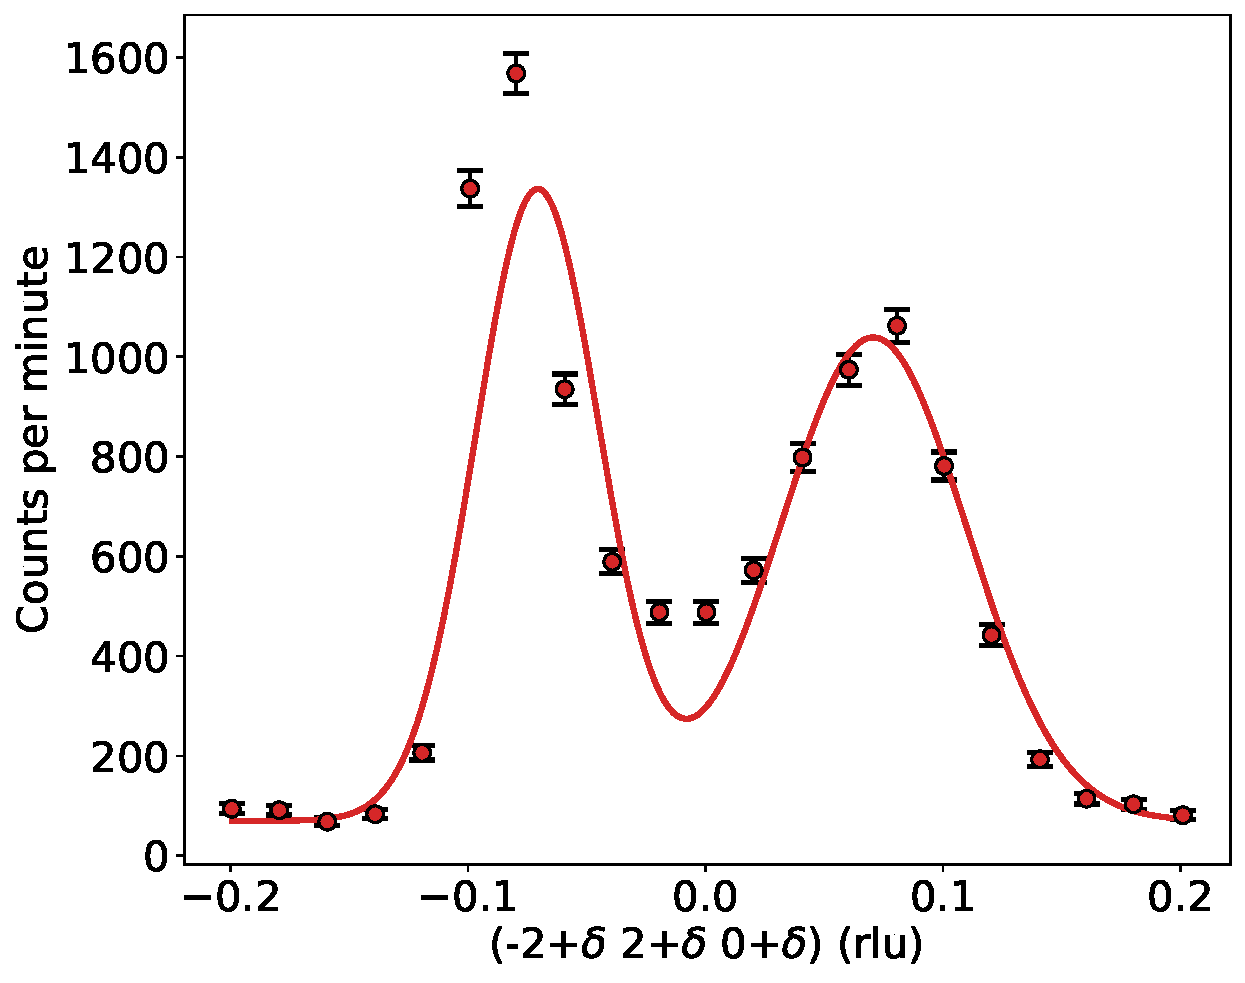
\includegraphics[width=1.0\linewidth]{energy-scan.pdf}
    \caption{\label{fig1} Constant energy scan at $\Delta E = 6.0\,\mathrm{meV}$ in [111] direction around (\bar{2}20). It shows the creation and annihilation peak of the phonon dispersion with the typical focusing and defocusing effect associated with the sloped resolution of a triple-axis spectrometer.}
\end{figure}

\begin{figure}
    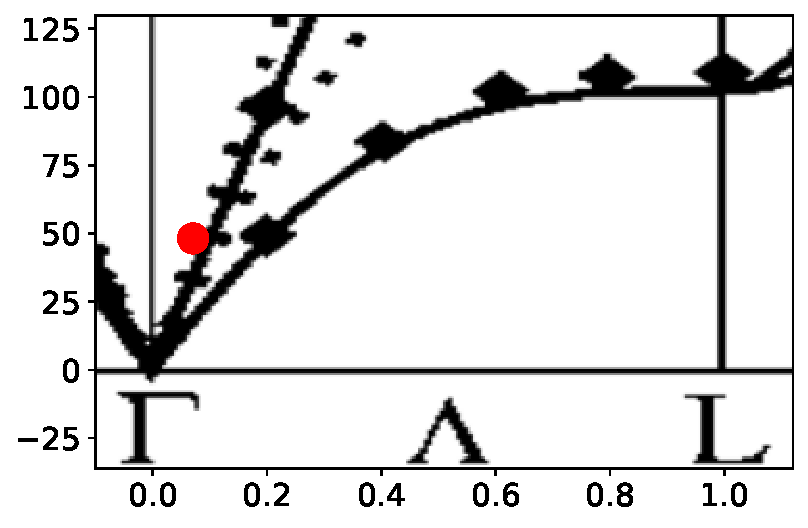
\includegraphics[width=1.0\linewidth]{dispersion.pdf}
    \caption{\label{fig2} Comparison of the data point we evaluated with the data previously published in \cite{Aouissi} }
\end{figure}



\section{Conclusions}

Summarize results...

This data analysis would have been much easier, if together with the data, some more information regarding the experiment would have been published, e.g. an experimental report or a lab book.


\begin{thebibliography}{9}

\bibitem{panosc} The Photon and Neutron Open Science Cloud (PaNOSC), \url{https://www.panosc.eu/}
\bibitem{nfdi} National research data infrastructure (NFDI), \url{https://www.dfg.de/en/research_funding/programmes/nfdi/index.html}
\bibitem{expands} European Open Science Cloud (EOSC) Photon and Neutron Data Service (ExPaNDS), \url{https://expands.eu/}
\bibitem{FAIR} FAIR principles, \url{https://www.go-fair.org/fair-principles/}
\bibitem{arXiv} arXiv.org, \url{https://arxiv.org/}
\bibitem{figshare} figshare, \url{https://figshare.com/}
\bibitem{IN3} IN3, \url{https://www.ill.eu/users/instruments/instruments-list/in3/description/instrument-layout/}
\bibitem{foster} Foster Open Data, \url{https://www.fosteropenscience.eu/}
\bibitem{mini-school} Czech-Bavarian mini-school on large scale facilities and open data \url{https://mini-school.eu/}
\bibitem{data} 
STEFFENS Paul; DELLEA Greta; DENG Yue; DIETL Christopher; DJURADO David; GAMBINO Marianna; HEPTING Matthias; INKINEN JUHO; JAFARI Atefeh; LEFRANCOIS Emilie; LOPES SELVATI Ana Carolina; PANAHI Hamed; PEDERSEN Martin Nors; PRADIP Ramu; RANIERI Umbertoluca; ROSSI Matteo; SCHATTE Sarah; STANA Markus; TIMOSENKO Janis; VONESHEN David and ZBIRI Mohamed. (2014). HSC17 Hercules practical course. Institut Laue-Langevin (ILL) doi:10.5291/ILL-DATA.TEST-2385 \url{doi:10.5291/ILL-DATA.TEST-2385}
\bibitem{Aouissi} Aouissi, M. and Hamdi, I. and Meskini, N. and Qteish, A; Phonon spectra of diamond, Si, Ge, and $\ensuremath{\alpha}\text{\ensuremath{-}}\mathrm{Sn}$: Calculations with real-space interatomic force constants; Phys. Rev. B, 74(5), 054302 (2006)

\end{thebibliography}

\end{document}
%
% ****** End of file apssamp.tex ******
